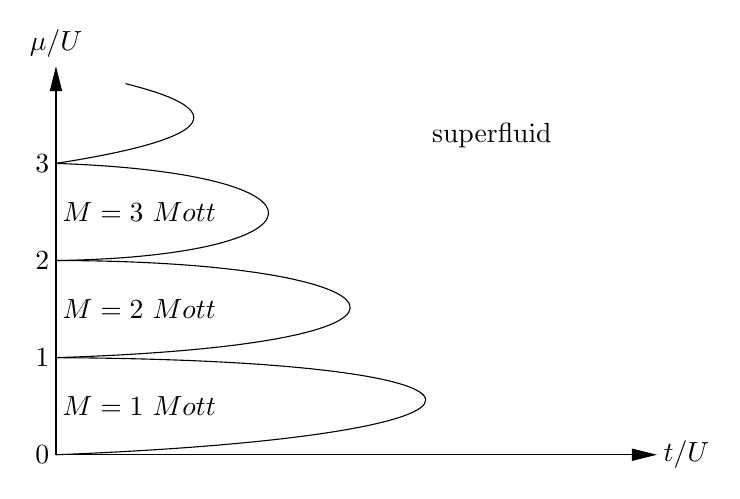
\begin{tikzpicture}[x=0.75pt,y=0.75pt,yscale=-1,xscale=1]
    %uncomment if require: \path (0,300); %set diagram left start at 0, and has height of 300
    
    %Straight Lines [id:da07533110977734148] 
    \draw    (112,245) -- (399.5,245) ;
    \draw [shift={(401.5,245)}, rotate = 180] [fill={rgb, 255:red, 0; green, 0; blue, 0 }  ][line width=0.08]  [draw opacity=0] (12,-3) -- (0,0) -- (12,3) -- cycle    ;
    %Straight Lines [id:da16123173761944054] 
    \draw    (112,245) -- (112,198.21) ;
    %Straight Lines [id:da25470462677223615] 
    \draw    (112,198.21) -- (112,151.42) ;
    %Straight Lines [id:da9203516859237628] 
    \draw    (112,151.42) -- (112,104.62) ;
    %Straight Lines [id:da8858272174506854] 
    \draw    (112,104.62) -- (112,59.83) ;
    \draw [shift={(112,57.83)}, rotate = 90] [fill={rgb, 255:red, 0; green, 0; blue, 0 }  ][line width=0.08]  [draw opacity=0] (12,-3) -- (0,0) -- (12,3) -- cycle    ;
    %Curve Lines [id:da690865334975969] 
    \draw    (112,245) .. controls (351.5,235.5) and (347.5,199.5) .. (112,198.21) ;
    %Curve Lines [id:da49915852555779927] 
    \draw    (112,198.21) .. controls (320.5,191.5) and (280.5,151.5) .. (112,151.42) ;
    %Curve Lines [id:da3871736130183383] 
    \draw    (112,151.42) .. controls (243.5,149.5) and (253.5,109.5) .. (112,104.62) ;
    %Curve Lines [id:da8267537682584203] 
    \draw    (112,104.62) .. controls (230.5,86.17) and (156.5,69.17) .. (145.5,66.17) ;
    
    % Text Node
    \draw (403.5,245) node [anchor=west] [inner sep=0.75pt]    {$t/U$};
    % Text Node
    \draw (112,54.83) node [anchor=south] [inner sep=0.75pt]    {$\mu /U$};
    % Text Node
    \draw (114,221.6) node [anchor=west] [inner sep=0.75pt]    {$M=1\ \text{Mott}$};
    % Text Node
    \draw (114,174.81) node [anchor=west] [inner sep=0.75pt]    {$M=2\ \text{Mott}$};
    % Text Node
    \draw (114,128.02) node [anchor=west] [inner sep=0.75pt]    {$M=3\ \text{Mott}$};
    % Text Node
    \draw (292,84) node [anchor=north west][inner sep=0.75pt]   [align=left] {superfluid};
    % Text Node
    \draw (110,198.21) node [anchor=east] [inner sep=0.75pt]   [align=left] {1};
    % Text Node
    \draw (110,151.42) node [anchor=east] [inner sep=0.75pt]   [align=left] {2};
    % Text Node
    \draw (110,104.62) node [anchor=east] [inner sep=0.75pt]   [align=left] {3};
    % Text Node
    \draw (110,245) node [anchor=east] [inner sep=0.75pt]   [align=left] {0};
    
    
    \end{tikzpicture}
    